
\subsection*{1.}

\(p(B) = 1 - p(A) = 1 - 0{,}40 = 0{,}60\).

\subsection*{2.}

\begin{center}
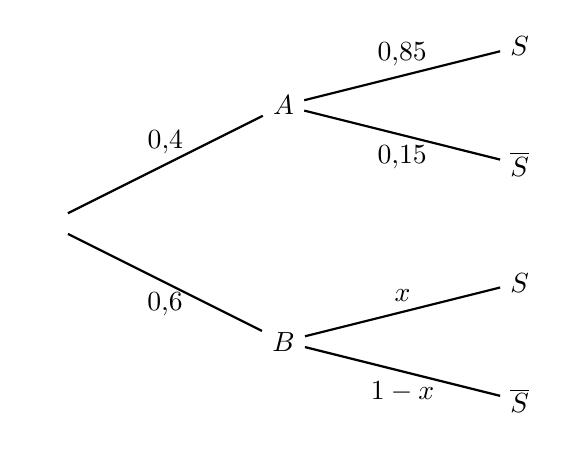
\begin{tikzpicture}[thick, scale=1.5]
\node (P_-1_0) at (-2,-1.5) {$\phantom{A}$};
\node (P_0_0) at (0,-0.5) {$A$};
\draw (P_-1_0) -- (P_0_0) node[midway, above] {$0{,}4$};
\node (P_1_0) at (2,-0) {$S$};
\draw (P_0_0) -- (P_1_0) node[midway, above] {$0{,}85$};
\node (P_1_1) at (2,-1) {$\overline{S}$};
\draw (P_0_0) -- (P_1_1) node[midway, below] {$0{,}15$};
\node (P_0_2) at (0,-2.5) {$B$};
\draw (P_-1_0) -- (P_0_2) node[midway, below] {$0{,}6$};
\node (P_1_2) at (2,-2) {$S$};
\draw (P_0_2) -- (P_1_2) node[midway, above] {$x$};
\node (P_1_3) at (2,-3) {$\overline{S}$};
\draw (P_0_2) -- (P_1_3) node[midway, below] {$1-x$};
\end{tikzpicture}
\end{center}

\subsection*{3.}

On doit trouver : \(p(A \cap S) = p(A) \times p_A(S) = 0{,}4 \times 0{,}85 = 0{,}34\).

\subsection*{4.}

On a, comme à la question \textbf{1.} : \(p(B \cap S) = p(B) \times p_B(S) = 0{,}6 \times x = 0{,}6x\).

D'après la loi des probabilités totales : \(p(S) = p(A \cap S) + p(B \cap S)\),

soit : \(0{,}91 = 0{,}34 + 0{,}6x\).

On en déduit : \(p(B \cap S) = 0{,}6x = 0{,}91 - 0{,}34\),

ou : \(p(B \cap S) = 0{,}6x = 0{,}57\).

On a donc : \(x = \dfrac{0{,}57}{0{,}60} = \dfrac{57}{60} = \dfrac{19}{20} = 0{,}95\).

\subsection*{5.}

Il faut trouver :
\[
p_S(B) = \dfrac{p(S \cap B)}{p(S)} = \dfrac{p(B \cap S)}{p(S)} = \dfrac{0{,}57}{0{},91} \approx 0{,}6263,
\]
soit \(0{,}626\) à \(10^{-3}\) près.

